The planned listening tests were performed on a total of twelve participants, of which ten were usable, with ages ranging from 21 to 30. There was some degree of confusion with regard to the features of the UI the participants were presented with, in particular the cubes used to mark which way the participant was facing. More than half of the subjects tested at least initially expected the sounds to come from these markers, and some mentioned that sounds continued to appear to originate from them even after they had been made aware of their purpose as just markers. In future tests, UI elements or position indicators should perhaps not have such a physical presence. A shortened version of the test was performed to allow the participants to acclimatise to the space, as well as to allow them to clarify any points of uncertainty before beginning the test proper. The tests themselves then took in between thirteen and nineteen minutes, and the primary bottleneck was the time spent preparing the next sample and fetching the modified HRTF data which was dependent on network speeds at the time. 

As mentioned in previous chapters, the primary metric for whether or not this implementation can be deemed effective is based upon the degree to which the severity of a participant's localisation errors decrease over time, if they decrease at all. This chapter will begin by investigating whether or not this is the case by reviewing the data captured during the listening tests. After this, further sections will investigate other conclusions or noteworthy observations that may be drawn from the additional data captured. Of particular interest is the aforementioned relationship between PCW adjustment and localisation, to this end I will be comparing PCW values and perceived/actual source positions before and after adjustment on an individual participant level.

\section{Localisation Error Over Time}
In order to properly analyse this metric I am looking at the average total error value for each of the eight source positions. This error value is the angular error that comes from subtracting the perceived source position from the actual source position. These two values are then made positive if either one is negative, so as to not produce deceptively low error values, and summed to produce a combined error value. This process is performed for every participant, and the mean error value for each measurement over the course of the test from each direction is then calculated based on that data. These mean error rates over time can then be plotted as in figure 4.1. 

\begin{figure}
	\caption{The average error rate over each direction.}
	\centering{
		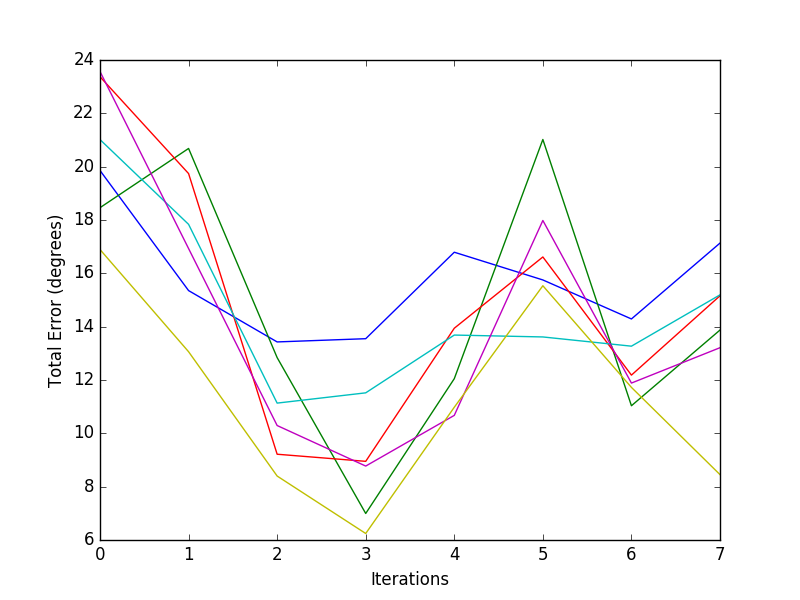
\includegraphics[scale=0.6]{average_error_each_direction}
	}
\end{figure}

On this chart each line represents a source position, and tracks how, on average, localisation errors for samples played from that source position changed over the course of the listening test. When displayed like this we can see something of a reduction in the overall errors for most source positions, but the short test length makes it unclear how close to zero these values would go or how long it would take - important considerations. What we can see at play is the self-correcting quality afforded to the algorithm through knowledge of the history of previous changes. For almost all of the directions there are large spikes where the algorithm explores a sub-optimal child state and the participant's subsequent localisation attempt fares more poorly, in all cases but one (the black line representing the [-45.0, 135.0] source position) this mistake is quickly rectified as the algorithm makes adjustments in the opposite direction. If successive child states could be selected more intelligently, then it's quite possible that these kinds of mis-steps could be minimized further, reaching a more effectively individualised HRTF sooner.

It's worth noting that three of the four directions with the most promising results were situated in front of the participant: [-45.0, 45.0], [45.0, 45.0], and [-45.0, -45.0]. This suggests a degree of front/back confusion in participants and a tendency towards assuming sources were positioned towards the front hemisphere of the test environment, leading to poor average error rates for sources positioned behind the participant. There is an exception to this in position [45.0, 135.0], which may have something to do with the starting HRTF used. Further research would be necessary to identify whether this is truly the case, but it would be interesting to see if it is possible to assemble an ideal base HRTF to begin this process with.

\section{Relationships Between PCs and Localisation Errors}
ignoring the lower order PCWs because they have a minimal effect
Looking for a connection between these two points essentially required finding a 

how did I look for this relationship? choosing the participant with the best performance and looking at their best source direction 

\bigskip

Steps involved, format PCWs into nice matrices and review them in sequence, viewing the direction of change and change value against the next perceived position

\bigskip 

Can we draw any conclusions from this? 

\section{•}
Then this structure could be repeated as needed, for as much analysis as I get to do??